\subsection{Experimental procedures}

\begin{frame}{Experimental settings}
\begin{itemize}
    \item Linear Algebra class. Selected topics: General Vector Space and Inner Product Space
    \item Fourteen concepts selected as predefined nodes
    \item Group formation: dyad (pair), selected freely by the students
    \item Location: computer laboratory
    \item Sit next to each other
\end{itemize}

\begin{figure}[tb]
        \begin{center}
            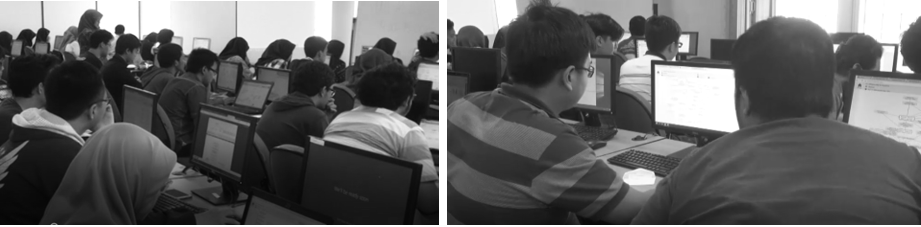
\includegraphics[width=100mm]{images/classroom_situation.pdf}
        \end{center}
        \caption{Classroom situation}
        \label{intro::rkb_p4}
    \end{figure}

\end{frame}

\begin{frame}{The learning activities during experiment}
\begin{table}[tb]
\begin{center}
\begin{tabular}{p{2.5cm}|p{5.5cm}|p{2cm}}%{c|c|c} %#{ | m{5em} | m{1cm}| m{1cm} | }
\hline
Phase & Students' Activity & Duration\\
\hline
Introduction & Kit-Build practice & 5 min.\\
Individual & (a) Create a concept map based on the predefined concepts (first map) & 25 min.\\
& (b) Create a re-constructional map based on the partner's first map components (second map) & 20 min.\\
Collaborative & (a) Discussion on shared and difference maps & 10 min.\\
& (b) Create a group concept map  (third map) & 30 min.\\
\hline
\end{tabular}
\end{center}
\caption{\label{tab:exp_setting} Timeline of students' activities during experiment}
\end{table}
 
{\tiny **Note: Three days after the experiment, the teacher gave feedback to the students.
The consent form to participate and a survey regarding students' affective response
toward the activities were also collected afterward. }

\end{frame}

\subsection{Participants and subject characteristics}

% \begin{frame}{Methods}

% \begin{itemize}
%   \item Participants and context of study
%   \item Experimental procedures
%   \item Data collection
% \end{itemize}

% \end{frame}

\begin{frame}{Participants}

\begin{itemize}
    \item Forty-four students of Linear Algebra class
    \item Majored in Computer Science or Information System at a public university in Indonesia
    \item 73\% of them are male students ($n = 32$)
    \item Most of them were the first year students in their second term
    \item They have experienced in various collaborative learning activities
    \item They used to create a concept map from scratch
\end{itemize}

\end{frame}
